%!TEX encoding = UTF-8

\documentclass[12pt, ULlof, ULlot]{ULrapport}

\usepackage[utf8]{inputenc}
\usepackage{float}


\TitreProjet{Projet de session}
\TitreRapport{Document de design}
\Destinataire{Philippe Voyer}
\NumeroEquipe{5}
\NomEquipe{Master Memers} %TODO: change this lol
\TableauMembres{%TODO: ajouter numéros de dossier
    111~107~781  & Maxime Ménard            & \\ \hline
    xxx~xxx~xxx  & Alexandre Turcotte       & \\ \hline
    xxx~xxx~xxx  & Julien Becirovski        & \\ \hline
}
\DateRemise{11 mars 2018}


\HistoriqueVersions{
     0    & 3 février 2018 & Création du document   \\ \hline
}

\begin{document}
    \section{Sommaire}
\label{s:sommaire}

    \section{Interactivité}
\label{s:interactivité}

Il y a deux modes d'interaction avec l'application: le clavier et la souris.
Le clavier est utilisé pour entrer des raccourcis permettant d'effectuer des actions alors que la souris permet de contrôler les éléments de l'interface graphique.

\subsection{Raccourcis clavier}
Les raccourcis clavier disponible sont les suivants:

\begin{table}[h]
    \begin{center}
    \begin{tabular}{|c|l|}
        \hline
        \multicolumn{1}{|c|}{Touche} & \multicolumn{1}{c|}{Action}\\
        \hline
        ctrl+Z / ctrl+Y & \emph{Undo} / \emph{Redo}\\
        Espace & Capture d'écran\\  
        Flèches gauche/droite & Rotation de la caméra autour de son axe Y local\\
        Flèches haut/bas & Rotation de la caméra autour de son axe X local\\
        A/D & Déplacement de la caméra sur son axe X local\\
        W/S & Déplacement de la caméra sur son axe Y local\\
        +/- & Déplacement de la caméra sur son axe Z local\\
        R & Réinitialisation de la pose de la caméra\\
        C & Changer le mode de projection de la caméra\\
        H & Afficher/cacher l'interface graphique\\
        1 & Créer une sphère\\
        2 & Créer un cube\\
        3 & Créer une ligne\\
        4 & Créer un triangle\\
        5 & Créer un rectangle\\
        6 & Créer un pentagone\\
        7 & Créer un cercle\\
        8 & Créer une flèche\\
        9 & Créer une étoile\\
        0 & Créer un mur en relief\\
        M & Créer un modèle 3D du Faucon Millenium\\
        X & Créer un modèle 3D d'un X-Wing Fighter\\
        P & Créer les deux portails\\
        B & Créer une courbe de Bézier\\
        N & Créer une courbe de Hermite\\
        E & Changer l'effet pleine fenêtre \\
        \hline
    \end{tabular}
    \caption{Raccourcis claviers de l'application}
    \end{center}
\end{table}
Il est à noter que les touches \emph{CTRL} droite et gauche fonctionnent pour les actions \emph{Undo} et \emph{Redo}.
De plus, le contrôle de la caméra s'effectue toujours dans son repère local.\\

\subsection{Interface graphique}
L'interface graphique comporte quatre panneaux.
Le premier est appelé \emph{Scène} et il se situe en haut à gauche de l'écran (voir figure \ref{fig:scene}).
Il affiche la liste des \emph{GameObjects} présents dans la scène.
Au démarrage de l'application, seule la lumière est présente, mais la liste se met à jour à chaque fois qu'on nouvel élément est ajouté à la scène.
Les objets sont affichés dans la liste dans l'ordre qu'ils sont créés et leur ordre n'est pas modifiable.
Il est possible de sélectionner un \emph{GameObjects} en cliquant sur le petit bouton à gauche de son nom dans la liste, ce qui modifie les autres panneaux de l'interface en conséquence.\\

\begin{figure}[H]
    \centering
	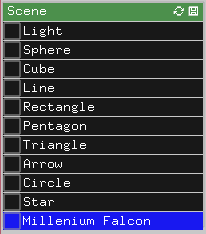
\includegraphics[scale=0.7]{fig/scene.png}
	\caption{Scène}
	\label{fig:scene}
\end{figure}

Le second panneau est appelé \emph{Inspecteur} et se situe à droite de l'écran (voir figure \ref{fig:inspecteur}).
Il permet de modifier les attributs du \emph{GameObject} présentement sélectionné.
Les attributs modifiables dans l'inspecteur dépendent du type de \emph{GameObject} qui est sélectionné.
Les différentes sections du chapitre sur les fonctionnalités présenteront quels attributs sont modifiables pour chaque type d'objet.\\

\begin{figure}[H]
    \centering
	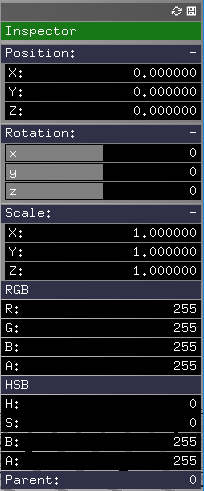
\includegraphics[scale=0.55]{fig/inspecteur.png}
	\caption{Inspecteur}
	\label{fig:inspecteur}
\end{figure}

Le troisième panneau de contrôle est celui des textures (voir figure \ref{fig:texture}).
Il s'affiche en bas à gauche de l'écran uniquement lorsqu'un \emph{GameObject} 2D (ligne, rectangle, triangle, cercle ou pentagone) est sélectionné.
Ce panneau permet de choisir la texture de l'objet 2D parmi les 5 textures procédurales offertes.

\begin{figure}[H]
    \centering
	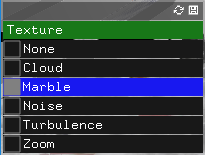
\includegraphics[scale=0.6]{fig/texture.png}
	\caption{Texture}
	\label{fig:texture}
\end{figure}

Le dernier panneau présent dans l'interface graphique est celui du mode d'éclairage (voir figure \ref{fig:mode_eclairage}).
Il s'affiche en bas à gauche de l'écran uniquement lorsque la lumière est sélectionnée.
Ce panneau permet de choisir parmi un des quatre types de lumière classiques, soient ponctuel, directionnel, projecteur et ambiant.

\begin{figure}[H]
    \centering
	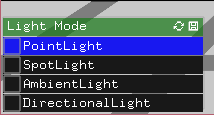
\includegraphics[scale=0.8]{fig/lightmode.png}
	\caption{Mode d'éclairage}
	\label{fig:mode_eclairage}
\end{figure}

Enfin, la seule sortie de l'application est une capture d'écran qu'il est possible d'effectuer en appuyant sur la barre espace (voir section \ref{ss:capture_ecran}).
\clearpage

    \section{Technologie}
\label{s:technologie}
L'environnement de développement du projet est composé du logiciel \textit{Visual Studio} et du framework \textit{openFrameworks}.
\subsection{Visual Studio}
Le développement de l'application se fait sur le système d'exploitation Windows pour toute l'équipe.
C'est donc naturellement que l'environnement de développement intégré \textit{Visual Studio} s'est imposé.
L'avantage est de pouvoir générer et configurer facilement un fichier projet pour que toute l'équipe de développement bénéficie de la même configuration de projet.
Il est aussi compatible avec le framework \textit{openFrameworks} qui nécessite l'installation d'une extension via le gestionnaire d'extension intégré et en ligne.
Aussi, \textit{openFrameworks} offre un générateur de projet compatible avec \textit{Visual Studio} permettant de créer une structure de projet vide et de gérer les add-ons dans les fichiers de configuration.

\subsection{openFrameworks}
L'application utilise le framework opensource \textit{openFrameworks} qui offre une interface haut-niveau avec la librairie de rendu 3D \textit{OpenGL}.
Ce framework offre plusieurs avantages dans le processus de développement dont le fait qu'il est distribué sur Windows, possède une communauté active qui fourni de la documentation et de nombreux tutoriels.
Ce aspect permet à l'équipe de développer dans un bon environnement avec des ressources disponibles. \\
\newline
Aussi, des add-ons sont utilisés pour aider à la création de l'interface graphique (\textit{ofxGui} et \textit{ofxInputField}) et l'importation de modèle 3D (\textit{ofxAssimpModelLoader}).

\subsection{Autres}
L'équipe a aussi utilisé le gestionnaire de version \textit{Git} pour le partage du code ainsi que \textit{Adobe Photoshop} pour le traitement des images.
\clearpage

    \section{Compilation}
\label{s:compilation}
    \section{Architecture}
\label{s:architecture}

\begin{figure}[H]
\centering
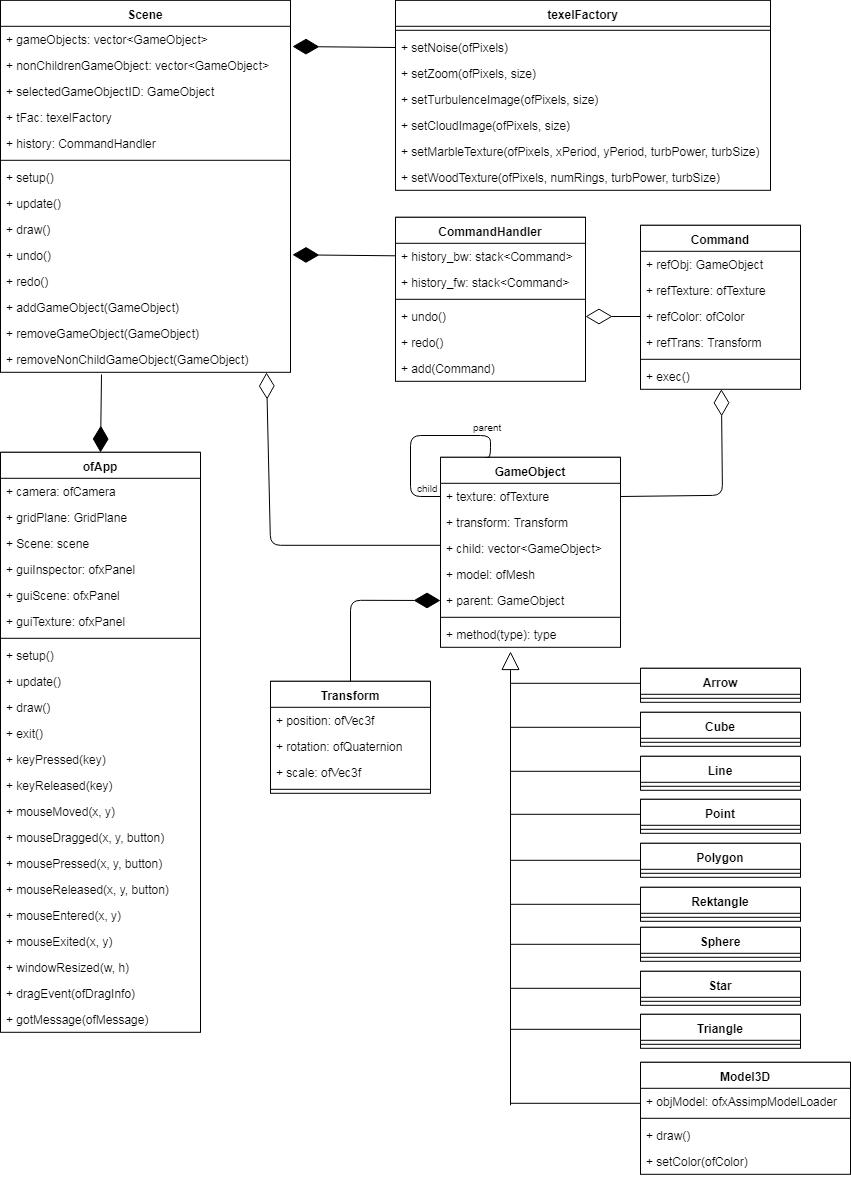
\includegraphics[width=0.85\textwidth]{img/INFOG-diagram-UML.png}
\caption{Diagramme UML}\label{fig-diagram-uml}
\end{figure}
    \section{Fonctionnalités}
\label{s:fonctionnalités}

\subsection{Image}
\subsubsection{Exportation d'image}
Il est possible d'exporter des rendus de la scène dans des fichiers PNG.
Pour ce faire, il suffit d'appuyer sur la barre espace et une capture d'écran de la fenêtre de l'application est sauvegardée dans le dossier \textit{/bin/data}.
Le fichier image est nommé en fonction de la date et de l'heure selon le format y$-$m$-$d\_hms.png.

\begin{figure}[H]
    \centering
	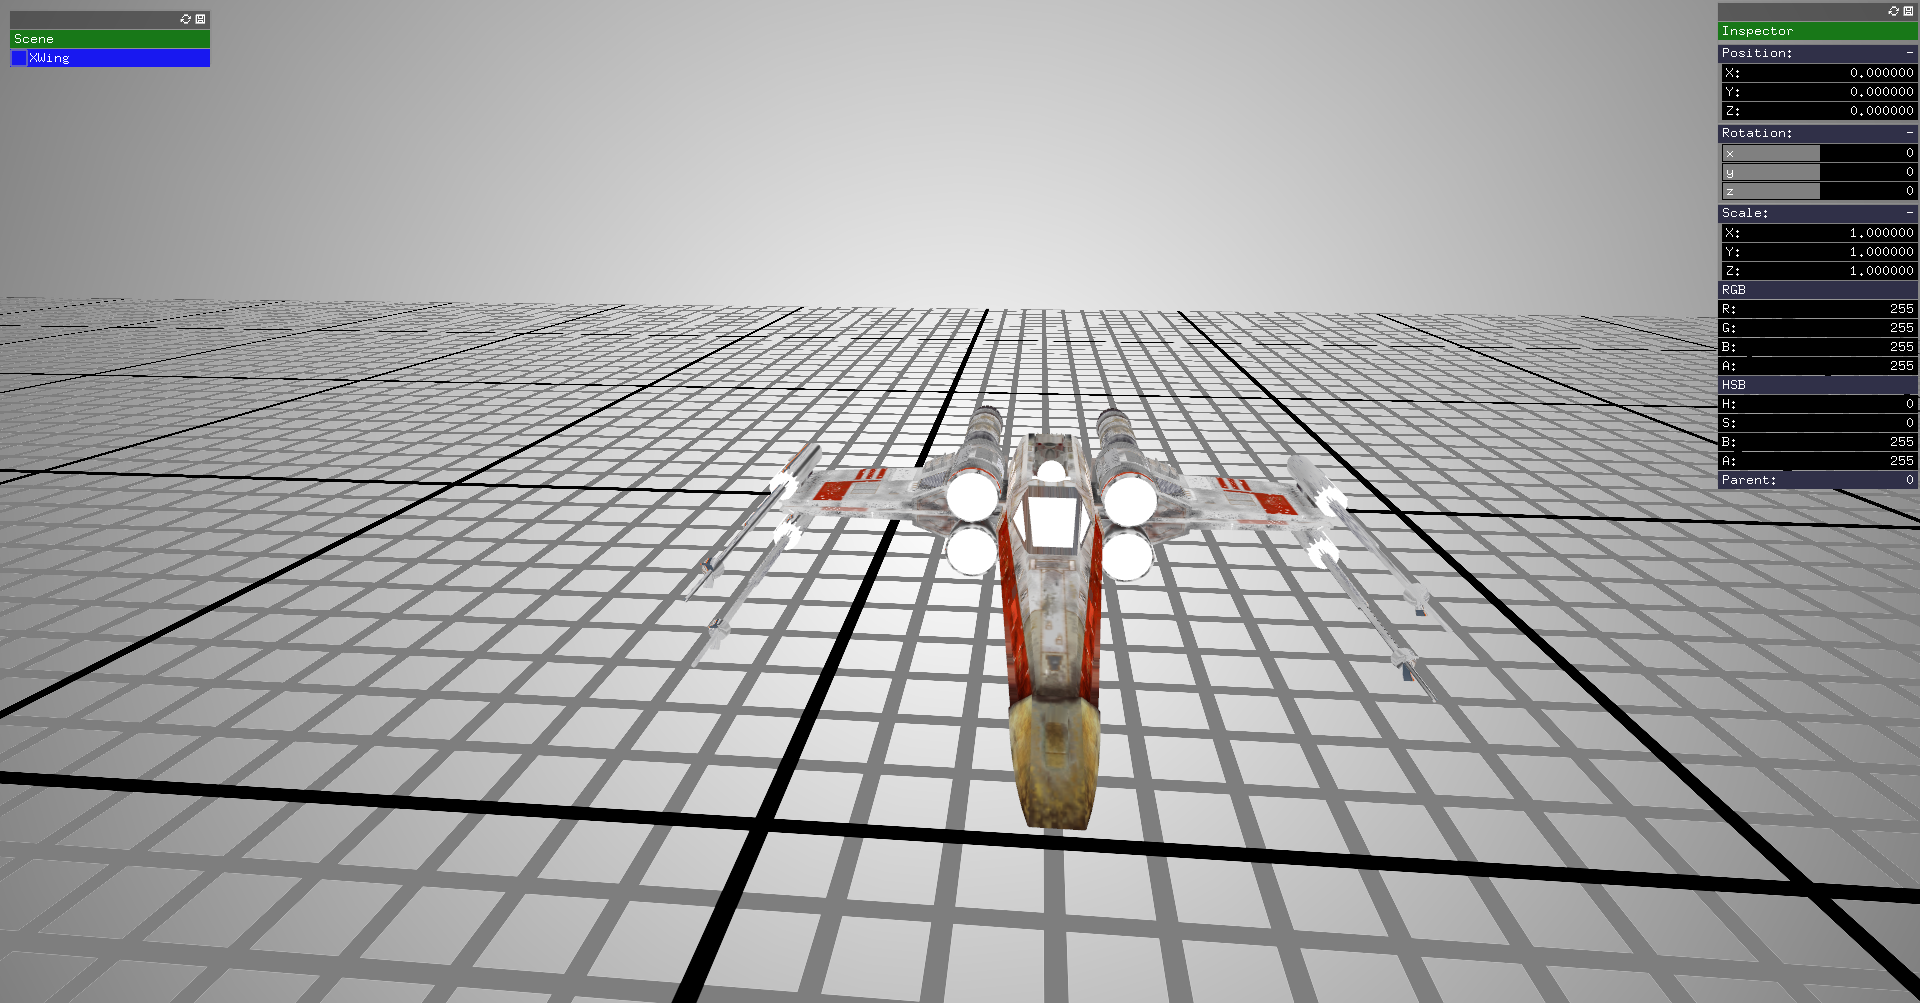
\includegraphics[scale=0.1]{fig/2018-3-11_22h34m38s.png}
	\caption{Exemple de capture d'écran}
	\label{fig:capture_ecran}
\end{figure}

\begin{figure}[H]
    \centering
	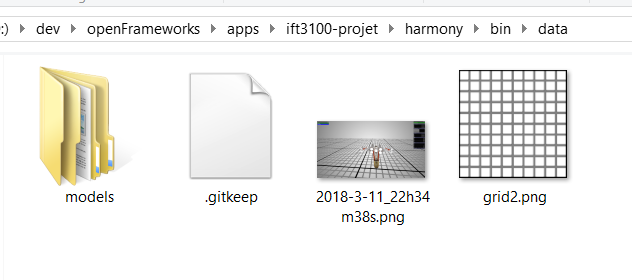
\includegraphics[scale=0.5]{fig/preuve-capture.png}
	\caption{Fichier exporté}
	\label{fig:preuve-capture}
\end{figure}

L'algorithme de capture d'écran est le suivant:
\begin{figure}[H]
    \centering
	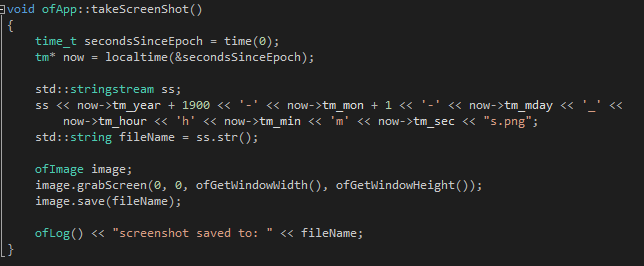
\includegraphics[scale=0.5]{fig/screenshotducodequiprenddesscreenshots.PNG}
	\caption{Code de la capture d'écran}
	\label{fig:capture_ecran}
\end{figure}

\subsubsection{Sélecteur de couleur}
\label{ss:selecteur_de_couleur}
L'inspecteur offre deux sélecteurs de couleurs affichant les valeurs des composantes de couleur de l'objet sélectionné et permettant de les modifier.
Chaque composante de couleur est encodée sur 8 bits, ce qui signifie que les sélecteurs acceptent des entiers entre 0 et 255.
\begin{figure}[H]
    \centering
	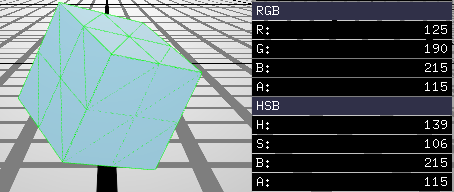
\includegraphics[scale=0.8]{fig/couleur.PNG}
	\caption{Sélecteurs de couleur}
	\label{fig:color_picker}
\end{figure}
Lorsque l'utilisateur entre une valeur dans un des champs, on récupère chacune des composantes et on applique cette couleurs à chaque vertex de l'objet sélectionné.

\subsubsection{Espace de couleur}
Un des sélecteurs de couleur de l'inspecteur permet de travailler en espace RGBA alors que l'autre permet de travailler en espace HSBA (voir la figure \ref{fig:color_picker}).
Lorsque la valeur d'une composante est modifiée dans un espace de couleur, l'autre sélecteur est mis à jour afin d'afficher les valeurs correspondantes.


\subsection{Dessin vectoriel}
\subsubsection{Primitives vectorielles}
Les primitives vectorielles offertes par cette application sont : une ligne, un triangle, un rectangle, un pentagone et un cercle.
Sur la figure suivante, on peut voir tous les objets qu'il est possible de créer dans l'application, incluant les primitives vectorielles.
\begin{figure}[H]
    \centering
	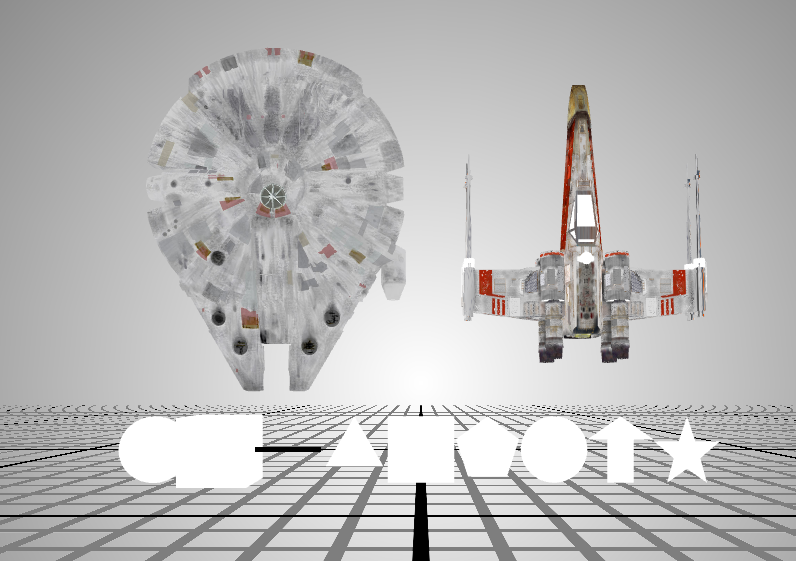
\includegraphics[scale=0.8]{fig/shapes.PNG}
	\caption{Formes 2D}
	\label{fig:primitives2D}
\end{figure}

\subsubsection{Forme vectorielle}
Les formes vectorielles offertes par cette application sont : une étoile et une flèche.
Sur la figure suivante, on peut voir tous les objets qu'il est possible de créer dans l'application, incluant les formes vectorielles.
\begin{figure}[H]
    \centering
	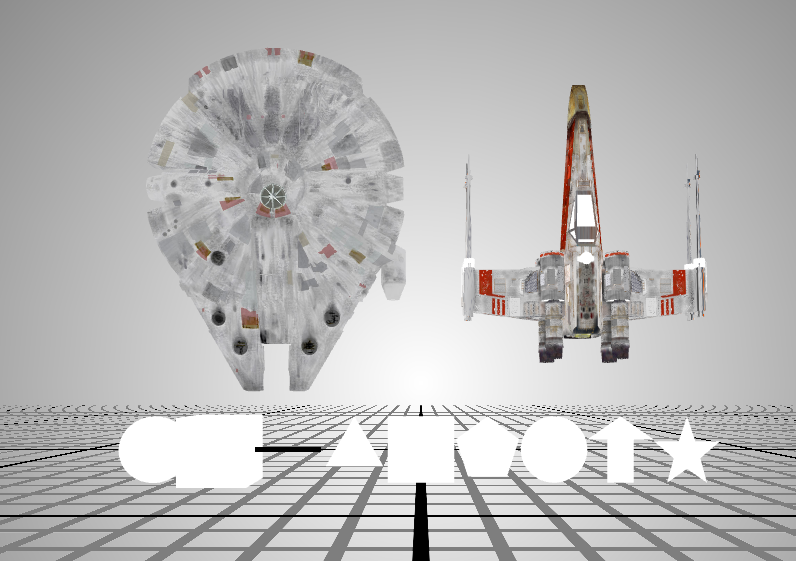
\includegraphics[scale=0.8]{fig/shapes.PNG}
	\caption{Formes 2D}
	\label{fig:formes2D}
\end{figure}

\subsubsection{Interface}
Nous avons décrit en grande majorité le fonctionnement de l’interface utilisateur et de ses éléments dans la section \ref{s:interactivité}.
Nous avons trois éléments d'interface graphique : l’inspecteur (pour modifier la position, la rotation, l’échelle de grandeur, la couleur et le parent des objets), le graphe de scène (voir tous les objets existant dans la scène ainsi que l’objet sélectionné) et l’interface de texture (offerte pour les objets 2D seulement, permettant de changer leur texture).
\begin{figure}[H]
    \centering
	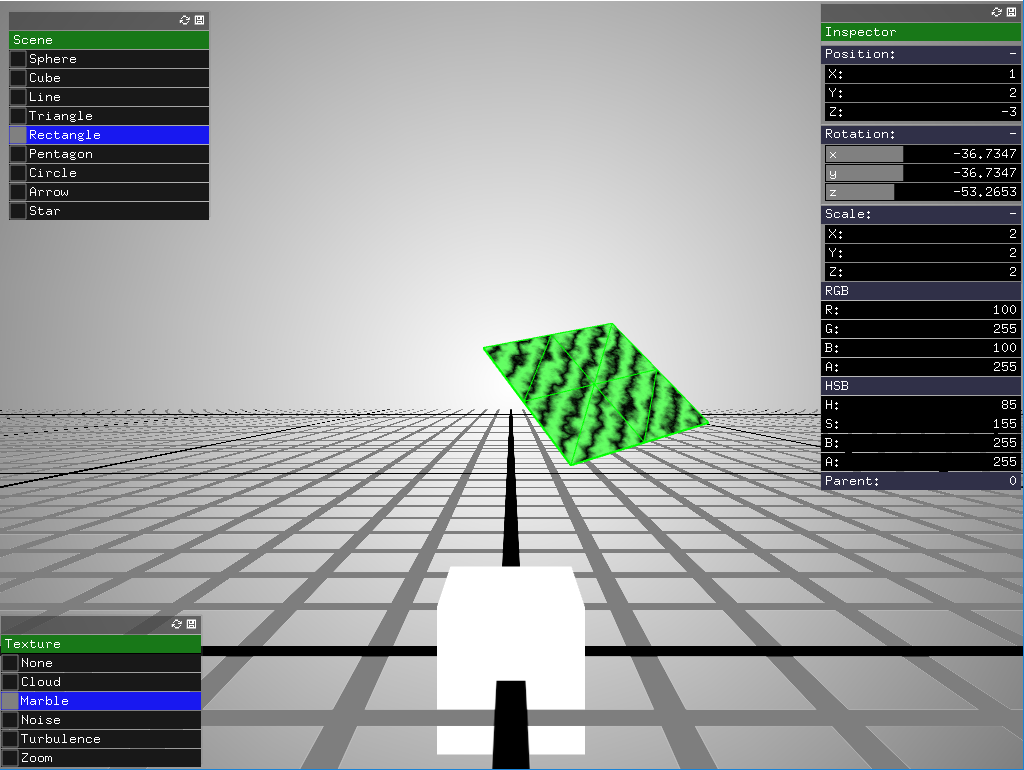
\includegraphics[scale=0.4]{fig/principale.PNG}
	\caption{Interface graphique}
	\label{fig:ui}
\end{figure}

\subsection{Transformation}
\subsubsection{Graphe de scène}
Le graphe de scène est une hiérarchie qui permet d’appliquer la transformation d’un parent sur ses objets enfants. On peut sélectionner un objet sur lequel on veut appliquer une transformation et il permet également de voir tous les éléments existant dans la scène. Pour plus d’information, voir \ref{fig:ui}.

\subsubsection{Transformations interactives}
L’interface utilisateur (le panneau Inspecteur) permet de façon interactive de changer la position, la rotation, la couleur, l’échelle de grandeur et le parent de l’objet sélectionné. Pour plus d’informations, se référer à \ref{fig:ui}.

\subsubsection{Historique des transformations}
\paragraph{} L'historique de transformation permet d'annuler et de récupérer une action provenant de l'utilisateur. Pour l'application, il est possible d'avoir l'historique du déplacement, de la rotation, de l'échelle et de la couleur pour chaque objet avec les touches \texttt{Ctrl+Z} et \texttt{Ctrl+Y}.
\paragraph{} L'état d'un objet \texttt{GameObject} est sauvegardé dans une classe \texttt{Command} à chacunes de ces actions. Le nombre de sauvegarde de commande est limité à 500. Cette commande est gérée par la classe \texttt{CommandHandler} qui s'occupe de sauvegarder les états courants (\texttt{CommandHandler::add()}), d'appliquer les changements d'état (\texttt{CommandHandler::undo()/redo()}) et d'ordonner les commandes dans deux \texttt{std::stack} dont une pour récupérer les commandes et une autre pour les annuler. Cette classe appartient à la classe \texttt{Scene} qui appelle la méthode de sauvegarde d'état à chaque fonction de modification d'un \texttt{GameObject}. Elle offre aussi les méthodes \texttt{Scene::undo()} et \texttt{Scene::redo()} pour que les événements puissent contrôler l'historique des transformations.

\subsection{Géométrie}
\subsubsection{Boîte de délimitation}
La boîte de délimitation permet de dessiner les arètes d’une boîte juste assez grande pour contenir les sommets d’un objet. Par contre, le Faucon Millénium et le « XWing » n’ont pas de boîte de délimitation car la position des sommets à l’intérieur du « mesh » est décalée par rapport au modèle 3D, ce qui dessinait la boîte très loin des objets eux-mêmes.
\begin{figure}[H]
    \centering
	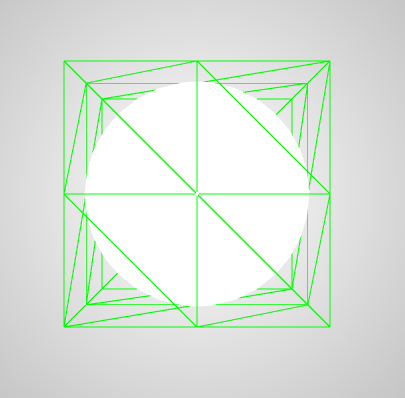
\includegraphics[scale=0.4]{fig/delimitation.PNG}
	\caption{Boîte de délimitation}
	\label{fig:box}
\end{figure}

\subsubsection{Primitives géométriques}
Les primitives géométriques offertes par cette application sont : un cube et une sphère.
Sur la figure suivante, on peut voir tous les objets qu'il est possible de créer dans l'application, incluant les primitives géométriques.
\begin{figure}[H]
    \centering
	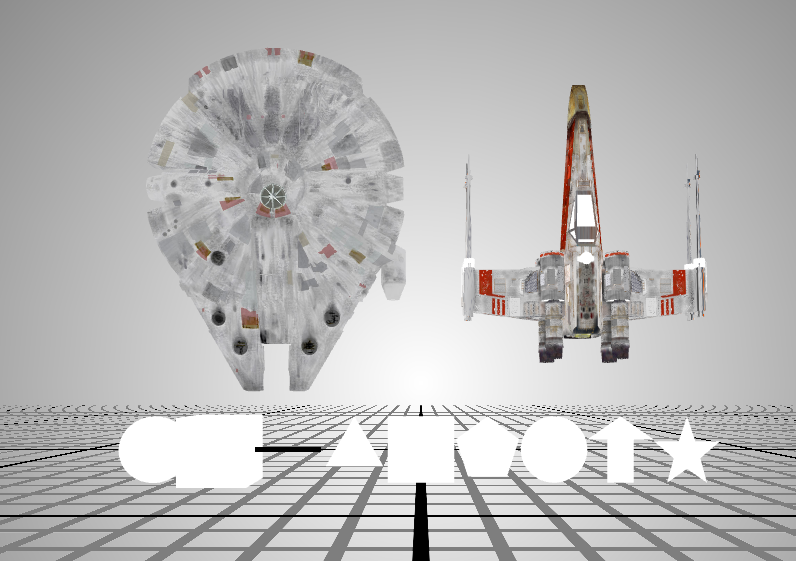
\includegraphics[scale=0.8]{fig/shapes.PNG}
	\caption{Primitives géométriques}
	\label{fig:primitivesgeo}
\end{figure}

\subsubsection{Modèle 3D}
Les modèles 3D offerts par cette application sont : le \textit{Faucon Millenium} et le \textit{X-Wing Fighter}.
Sur la figure suivante, on peut voir tous les objets qu'il est possible de créer dans l'application, incluant les modèles 3D.
\begin{figure}[H]
    \centering
	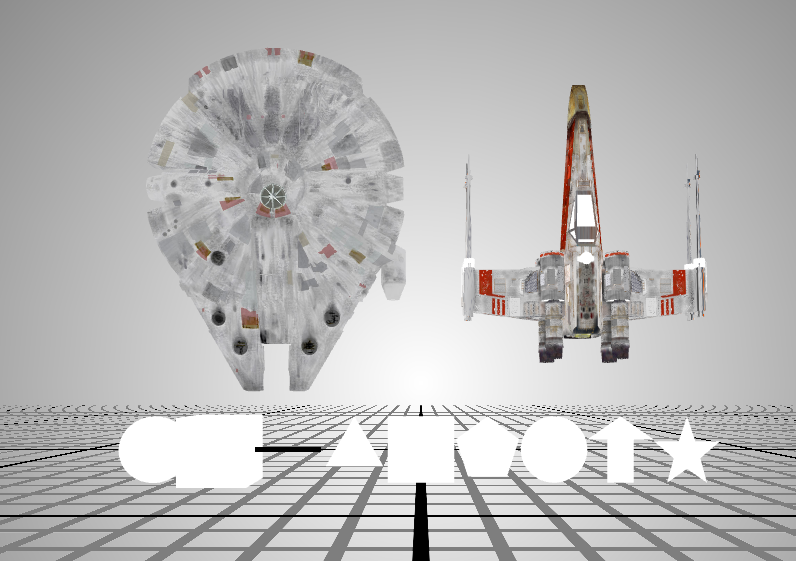
\includegraphics[scale=0.8]{fig/shapes.PNG}
	\caption{Modèles 3D}
	\label{fig:modeles3D}
\end{figure}

\subsection{Texture}
\subsubsection{Mapping}
Les modèles 3D du \textit{Faucon Millenium} ainsi que du \textit{X-Wing Fighter} sont texturés avec des coordonnées de mapping contenues dans leur fichier .OBJ respectif.
Le add$-$ons \textit{ofxAssimpModel} permet de charger ces modèles et s'occupe de créer les coordonnées de textures correspondant à chaque sommet.
Sur la figure suivante, on peut voir les deux modèles avec leur texture appliquée adéquatement.
\begin{figure}[H]
    \centering
	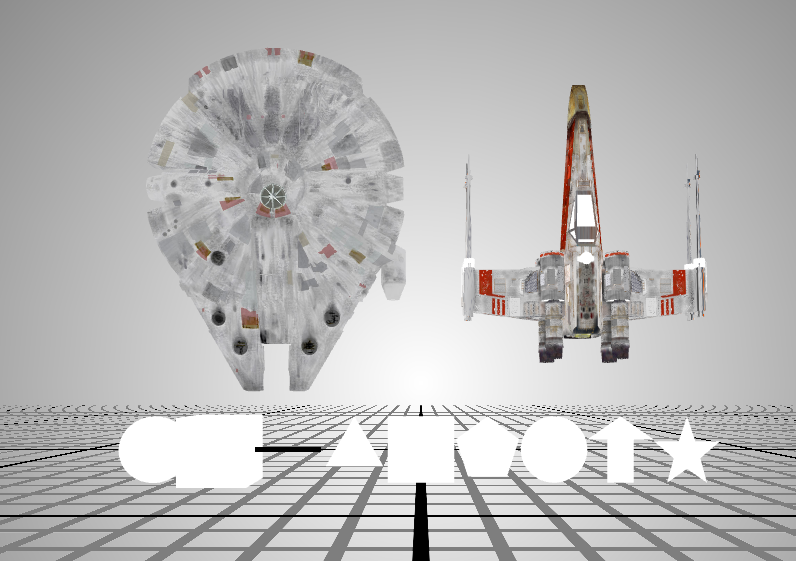
\includegraphics[scale=0.4]{fig/shapes.PNG}
	\caption{Modèles 3D texturés}
	\label{fig:mapping}
\end{figure}

Chaque forme 2D qu'il est possible de créer (ligne, rectangle, triangle, cercle, pentagone, flèche et étoile) possède des coordonnées de texture permettant de leur associer les textures procédurales.
Par exemple, la figure suivante montre l'étoile texturée.
\begin{figure}[H]
    \centering
	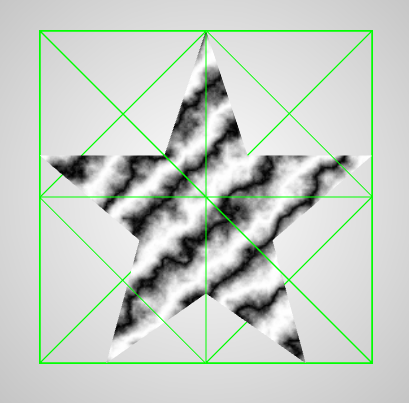
\includegraphics[scale=0.4]{fig/star.PNG}
	\caption{Étoile texturée}
	\label{fig:mapping2}
\end{figure}



\subsubsection{Texture procédurale}
\paragraph{} Les textures procédurales proviennent d'un patron de base sur lequel est appliqué des algorithmes. Les patrons de bases utilisés sont le bruit de perlin, le patron en sinus et le patron en cercle.
\paragraph{} Il est possible de générer une texture procédurale imitant l'effet nuage avec le bruit de perlin, une interpolation linéaire, un algorithme de turbulence et une modification les paramètres HSL. L'effet marbre est généré par le patron en sinus sur lequel on applique un algorithme de turbulence. L'effet bois est généré par le patron en cercle sur lequel on applique un algorithme de turbulence ainsi qu'un filtre de couleur bois (orangé / brun).
\begin{figure}[H]
\centering
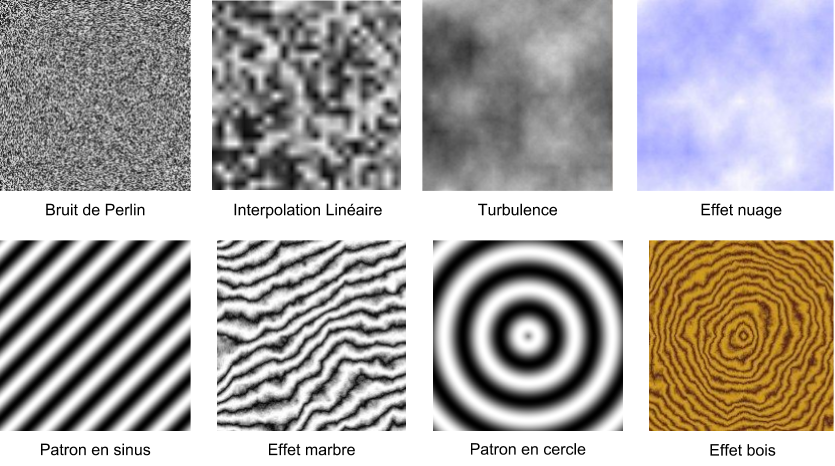
\includegraphics[width=\textwidth]{img/infog-image-procedural-texture.png}
\caption{Textures procédurales}\label{fig-procedural-texture}
\end{figure}
\paragraph{} Au niveau de l'application, une classe \texttt{texelFactory} s'occupe de générer toutes les textures procédurales présentées plus-haut (\ref{fig-procedural-texture}).  Chaque textue est interfacée par une méthode permettant de transformer un buffer \texttt{ofPixels} avec des paramètres (puissance de la turbulence par exemple) qui seront utilisées par les algorithmes correspondants (réf. \ref{src-procedural-texture}). Par la suite, ce buffer est appliqué sur le \texttt{GameObject} qui possède un \texttt{ofTexture} et un \texttt{ofMesh} propre. Aussi, lors de la création du \texttt{ofMesh}, il est nécessaire de cartographier la texture sur la forme avec la méthode \texttt{ofMesh::addTextCoord} et \texttt{ofTexture::getCoordFromPercent}.

%%%%%%%%%%%%%%      TP2      %%%%%%%%%%%%
% >> CAMÉRA
\subsection{Caméra}
\subsubsection{xxx}

% >> ILLUMINATION
\subsection{Illumination}
\subsubsection{Modèle d'illumination}

% >> LANCER DE RAYON
\subsection{Lancer de rayon}
\subsubsection{xxx}

% >> TOPOLOGIE
\subsection{Lancer de rayon}
\subsubsection{xxx}

% >> TECHNIQUE DE RENDU
\subsection{Techniques de rendu}
\subsubsection{Effet en pleine fenêtre}
Les effets en pleine fenêtre sont gérés par la classe \texttt{fboRender}. Cette classe permet d'appliquer 3 types d'effet visuel dont un effet \textbf{flou gaussien}, un effet \textbf{noir et blanc} et un effet \textbf{sépia}. Il est possible de passer d'un effet à un autre avec la touche \textbf{'e'} lorsque le logiciel est lancé.

\begin{figure}[H]
    \centering
	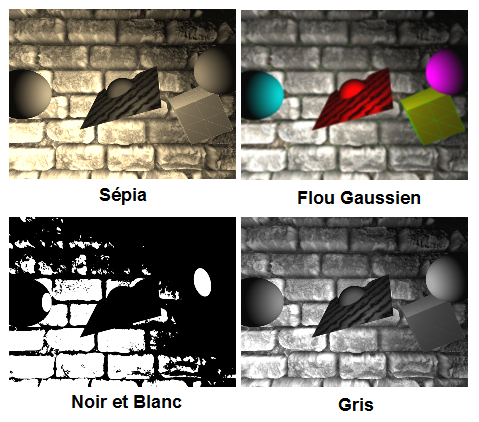
\includegraphics[scale=0.8]{img/infog-image-effet-plein-ecran.png}
	\caption{Application des effets sur la scène en cours.}
	\label{fig:effects}
\end{figure}

Chaque effet est géré par son propre shader qui se trouve dans le dossier \texttt{bin/data/shaders} qui contient les fichiers \textit{Vertex Shader} et \textit{Fragment Shader}. Le principe est de dessiner la scène dans un élément \texttt{ofFbo} pour rastériser le plan image afin d'appliquer par la suite les \texttt{shaders} appropriés. Ensuite, on dessine l'objet \texttt{ofFbo} pour afficher le résultat à l'écran.


\subsubsection{Effet de relief}

\subsubsection{Style libre}
    \section{Ressources}
\label{s:ressources}

La seule ressource originale produite par l'équipe est l'image \textit{grid2.png} située dans le dossier \textit{/bin/data}.
Il s'agit d'une grille 10x10 avec transparence qui a été réalisée dans \textit{Adobe Photoshop}.\\

Les modèles 3D du \textit{Faucon Millenium} ainsi que du \textit{X-Wing Fighter} utilisés dans l'application ont été trouvés sur le site \url{https://free3d.com/free-3d-models/obj}.
Le modèle du Faucon Millenium a été produit par A. Meerow et est la propriété de Disney/LucasFilm.
Le modèle du X-Wing Fighter a été produit par Glenn Campbell, Harry Chang, Jose Gonzales Pareja, Matt Walton ainsi que Matt Allen et est la propriété de Disney/LucasFilm.
Ces deux modèles 3D doivent être utilisés à des fins personnelles seulement.
Ils se trouvent dans le dossier \textit{/bin/data/models}.\\ 

Le code des textures procédurales s'inspire du site \textit{Texture Generation using Random Noise}, (Lode Vandevenne, 2004) \url{http://lodev.org/cgtutor/randomnoise.html}.
\label{src-procedural-texture}

    \section{Présentation}
\label{s:présentation}

\subsection{Maxime Ménard}
Je suis étudiant en quatrième année en génie informatique avec une concentration en systèmes intelligents.
J'ai contribué par le passé au projet Robocup Ulaval et je suis présentement responsable de l'équipe logicielle du Groupe Aérospatial de l'Université Laval (GAUL).
Dans ce projet, j'ai mis en place la structure du projet et l'architecture logicielle.
J'ai également travaillé sur la transformation et le rendu des objets, les courbes paramétriques, la lumière, les portails et l'interface graphique.

\subsection{Alexandre Turcotte}
Je suis à ma première année universitaire, soit à ma deuxième session, en IFT avec une passerelle DEC-BAC.
Je suis également en concentration de jeux-vidéo, et donc plus tard mon but est d’être programmeur ou designer de jeux-vidéo.
J’ai fait plusieurs projets personnels, mon plus récent étant un clone de League of Legends qui me permettra de développer des personnages par moi-même et de les tester au lieu de simplement les faire sur papier.
Dans ce travail, j’ai principalement travaillé sur l’interface utilisateur et ses fonctionnalités ainsi que sur les relations parents-enfants, les modes de projection de la caméra, les portails ainsi que sur les matériaux.

\subsection{Julien Becirovski}
Je suis étudiant en dernière année de génie informatique avec une concentration en robotique mobile et leurs applications. J'ai choisi d'effectuer mon dernier cours de concentration en infographie dans le but de comprendre et d'appliquer les technologies liées au rendu 3D qui sont notamment utilisées dans les simulateurs. Dans ce projet, je travaille sur les textures procédurales, le mappage des textures sur les primitives vectorielles 2D, l'historique de transformation, les modèles d'illumination et le rendu.
\clearpage

\end{document}
